\documentclass[11pt;a4paper]{report}
\usepackage[free-standing-units]{siunitx}
\usepackage{circuitikz}
\usepackage{tikz}
\usepackage[utf8]{inputenc}
\usepackage{fontenc}
\usepackage[french]{babel}
\usepackage{lmodern}
\usepackage{amsmath}
\usepackage{amssymb}
\usepackage{mathrsfs}
\usepackage[top=2cm, bottom=2cm, left=2cm, right=2cm]{geometry}
\usepackage{multirow}
\usepackage{url,hyperref}
\usepackage{siunitx}
\usepackage{schemabloc}

\title{
\includegraphics{../../../../images/inp-enseeiht} \\ ~ \\ ~ \\ ~ \\ ~ \\ Mini Projet Électronique Linéaire \\ ~ \\ \large{Réalisation d'un amplificateur de tension}}
\author{Mathieu Couffinhal, Guilhem Saurel}
\date{\oldstylenums{\today}}

\renewcommand{\thechapter}{\Roman{chapter}}
\renewcommand{\thesection}{\thechapter .\Alph{section}}

\includeonly{2}
\begin{document}
 \begin{titlepage}
  \maketitle
 \end{titlepage}


 %\hspace{30mm}
 \tableofcontents
  \chapter{Énoncé}
  \section{Cahier des charges}

    \begin{tabular}{|l|l|c|c|c|c|c|}
     \hline
     & & Typique & Tolérance & Minimum & Maximum & Unités \\
     \hline
     \multirow{4}{3cm}{Caractéristiques générales à 30k\hertz} & Gain en tension & 60 & $\pm$ 5dB & 55 & 65 & dB \\
     \cline{2-7} & Résistance d'entrée & 30 & $\pm$ 15 \% & 25.5 & 34.5 & \kilo\ohm \\
     \cline{2-7} & Résistance de sortie & 100 & $\pm$ 15 \% & 85 & 115 & \ohm \\
     \cline{2-7} & Dynamique de sortie (5\kilo\ohm)& & & 6 & & V càc \\
     \cline{2-7} & Dynamique de sortie (100\ohm)& & & 0.1 & & V càc \\
     \hline
     \multirow{2}{3cm}{Fréquence de coupure} & basse & 100 & $\pm$ 20 \% & 80 & 120 & \hertz \\
     \cline{2-7} & haute & & & 500 & & k\hertz \\
     \hline
     Distorsion harmonique & [1k\hertz;100k\hertz] & & & & 5,00 \% & \\
     \hline
     \multirow{2}*{Tension d'alimentation} & Positive & 12V & & 0 & 12 & V \\
     \cline{2-7} & Négative & -12V & & -12 & 0 & V \\
     \hline
     Courant de collecteur & & & & 0.1 & 10 & mA \\
     \hline
    \end{tabular}


  \section{Contraintes}
    Obligation d'utiliser un montage d'amplification différentiel.

    Consommer le moins possible.


  \section{Conditions d'utilisation}

    \underline{Entrée} : Générateur basse fréquence de résistance interne $R_g = 50 \ohm$

    \underline{Sortie} : Résistance de charge $R_L = 5\kilo\ohm$


  \section{Composants}
    \underline{Actifs} : Transistors BC238

    \underline{Passifs} : Composants appartenant à la norme E12

    \underline{Valeurs} de la norme E12 : 1 ; 1.2 ; 1.5 ; 1.8 ; 2.2 ; 2.7 ; 3.3 ; 3.9 ; 4.7 ; 5.6 ; 6.8 ; 8.2

    \begin{tabular}{|c|c|c|c|}
     \hline
     & Minimum & Maximum & Unités \\
     \hline
     Résistances & 10 & $10^6$ & \ohm \\
     \hline
     Condensateurs & 10 & $4,7.10^6$ & pF \\
     \hline
    \end{tabular}

    Précisions : À partir de 1 $\micro$F, les condensateurs sont polarisés ( ils ont donc un sens de branchement). 
    Les seules valeurs disponibles sont 1$\micro$F, 2.2$\micro$F et 4.7$\micro$F.

  \chapter{Études théorique des différents composants}
  \section{Collecteur Commun}
   \subsection{Schéma}

   On utilisera le schéma suivant de collecteur commun :

    \begin{circuitikz} \draw
     (0,3) to[open,v=$V_E$] (0,-2)
     (6,0) to[open,v=$V_S$] (6,-2)
     (0,-2) -- (6,-2)
     (0,3) to[C=$C_i$,i=$I_E$] (2,3)
      to [R=$R_{B1}$] (2,6) -- (4,6)
      to [R=$R_C$] (4,4)
     (4,3) node[npn](npn){}
      (npn.B) -- (2,3)
      (npn.C) -- (4,4)
      (npn.E) -- (4,2)
     (2,3) to [R=$R_{B2}$] (2,-2) -- (4,-2)
      to [R=$R_{E2}$] (4,0)
      to [R=$R_{E1}$] (4,2)
     (4,0) to [C=$C_o$,i=$I_S$] (6,0)
     (1,6) node[anchor=east] {$V_{cc}$} to [short,o-] (2,6)
     ;
    \end{circuitikz}

   \subsection{Polarisation}
    En raison de la présence des condensateurs, ce circuit est équivalent à (en continu) :

    \begin{circuitikz} \draw
        (3,2) to [R=$R_{E1}$] (3,0) 
      to [R=$R_{E2}$] (3,-2) -- (0,-2)
      to [battery=$E_{th}$] (0,3)
      to [R=$R_B$] (2,3)
     (2,6) node[anchor=east] {$V_{cc}$} to [short,o-] (3,6)
      to [R=$R_C$] (3,4)
     (3,3) node[npn](npn){}
      (npn.B) -- (2,3)
      (npn.C) -- (3,4)
      (npn.E) -- (3,2)
     ;
    \end{circuitikz}

    On a alors les relations suivantes :

    $\left.
      \begin{array}{c}
       R_B = \cfrac{R_{B1} R_{B2}}{R_{B1} + R_{B2}} \\
       E_{th} = \cfrac{V_{cc}}{1+\cfrac{R_{B1}}{ R_{B2}}} \\
       R_E I_C + V_{BE} + R_B I_B = E_{th} \\
       I_C = \beta I_B
      \end{array}
    \right\} \Rightarrow I_C = \cfrac{E_{th} - V_{BE}}{R_E + \cfrac{R_B}{\beta}}$

   \subsection{Droite de charge statique}

    Afin de limiter les effets de distorsion, on s'efforcera de placer le point de polarisation Q au milieu de la droite de charge statique.
    
    $V_{cc} = R_C I_C + V_{CE} + R_E I_C$

    $I_C = \cfrac{V_{cc} - V_{CE}}{R_E+R_C}$

    \begin{circuitikz}
     \begin{scope}[xshift=6.5cm, yshift=.5cm]
      \draw [->] (0,0) -- (4.5,0) node[anchor=west] {$V_{CE} $};
      \draw [->] (0,0) -- (0,2.5) node[anchor=west] {$I_C$} ;
      \draw (2,0) node[anchor=north] {$\cfrac{V_{cc}}{2}$}
            (4,0) node[anchor=north] {$V_{cc}$}
            (0,1) node[anchor=east] {$\cfrac{V_{cc}}{2(R_E+R_C)}$}
            (0,2) node[anchor=east] {$\cfrac{V_{cc}}{R_E+R_C}$}
            (0,0) node[anchor=north] {0};
      \draw [thick] (0,2) -- (4,0);
      \draw [dotted] (0,1) -- (2,1) -- (2,0);
     \end{scope}
    \end{circuitikz}

   \subsection{Schéma équivalent petit signal}
    Aux fréquences moyennes et en comportement petit signal, on obtient le schéma équivalent suivant :

    \begin{circuitikz} \draw
     (0,4) to[open,v=$V_E$] (0,-2) -- (11,-2)
     (11,0) to[open,v=$V_S$] (11,-2)
     (0,4) to [short,i=$I_E$] (1,4) --(5,4)
      to [R=$r_b$,v=v] (5,2) -- (9,2)
     (1,-2) to [R=$R_{B1}$] (1,4)
     (3,-2) to [R=$R_{B2}$] (3,4)
     (9,-2) to [R=$R_{E2}$] (9,0)
     (9,0) to [R=$R_{E1}$] (9,2)
     (7,-2) to [cI=$g_mv$] (7,2)
     (9,0) to [short,i=$I_S$] (11,0)
     ;
    \end{circuitikz}

    $g_m = \cfrac{I_C}{U_T}$

    $r_b = \cfrac{\beta}{g_m}$

   \subsection{Droite de charge dynamique}

    $\cfrac{V_{CE}(t)}{I_C(t)} = - R_E \parallel Z_L$

    \begin{circuitikz}
    \begin{scope}[xshift=6.5cm, yshift=.5cm]
     \draw [->] (0,0) -- (4.5,0) node[anchor=west] {$V_{CE}(t) $};
     \draw [->] (0,0) -- (0,2.5) node[anchor=west] {$I_C(t)$} ;
     \draw (3,0) node[anchor=north] {$V_{CE_Q}$}
           (4,0) node[anchor=north] {$V_{CE_{max}}$}
           (0,0.5) node[anchor=east] {$I_{C_Q}$}
           (0,2) node[anchor=east] {$I_{C_{max}}$}
           (0,0) node[anchor=north] {0};
     \draw [thick] (0,2) -- (4,0);
     \draw [dotted] (0,0.5) -- (3,0.5) -- (3,0);
    \end{scope}
    \end{circuitikz}

    Donc dynamique de sortie maximale (crête à crête) = $2(V_{CEmax}-V_{CEQ}) = 2 I_{CQ} (R_E \parallel Z_L)$ car $V_S = -V_{CE}$

   \subsection{Impédance d'entrée}

    $\left.
     \begin{array}{c}
      Z_E = \cfrac{V_E}{I_E}\\
      V_E = v + V_S \\
      v = r_b i \\
      V_S = (R_E \parallel Z_L)(i+g_mv)
     \end{array}
    \right\} 
    \begin{array}{l}
     \Rightarrow \cfrac{V_E}{i}=\cfrac{v+V_S}{i} =r_b + (R_E\parallel Z_L)(1+g_mr_b) \\
     \Rightarrow Z_E = R_B \parallel \left ( r_b + \beta (R_E\parallel Z_L) \right )
    \end{array}$

   \subsection{Impédance de sortie}

    $Z_S = R_{E2} \parallel \left(R_{E1}+\cfrac{r_b + R_g \parallel R_B}{\beta}\right)$

   \subsection{Gain}

    $a_v = \cfrac{V_S}{V_E} = \cfrac{V_S}{v+V_S} = \cfrac{\beta(R_E \parallel Z_L)}{r_b+\beta(R_E\parallel Z_L)} \approx 1$

    ~

    On considérera donc le gain de cet étage comme égal à 1.

   \subsection{Comportement en fréquence}
    «À vue», l’influence de $C_i$ intervient dans la fonction de transfert
    
    $H = \cfrac{Z_E}{Z_E+R_g}\cdot\cfrac{(Z_E+R_g)C_ip}{1+(Z_E+R_g)C_ip}$, 

    donc $f_{CBF1} = \cfrac{1}{2\pi(Z_E+R_g)C_i}$

    On étudie l’influence de $C_o$ de la même manière:

    $H = \cfrac{Z_L}{Z_L+Z_S}\cdot\cfrac{(Z_L+Z_S)C_ip}{1+(Z_L+Z_S)C_ip}$, 

    donc $f_{CBF2} = \cfrac{1}{2\pi(Z_L+Z_S)C_i}$

  \section{Émetteur Commun Dégénéré}
   \subsection{Schéma}
    On utilisera le montage émetteur commun suivant :

    \begin{circuitikz} \draw
     (0,3) to[open,v=$V_E$] (0,-2)
     (7,4) to[open,v=$V_S$] (7,-2)
     (0,-2) -- (7,-2)
     (0,3) to[C=$C_i$,i=$I_E$] (2,3)
      to [R=$R_{B1}$] (2,6) -- (4,6)
      to [R=$R_C$] (4,4)
      to [C=$C_o$,i=$I_S$] (7,4) 
     (4,3) node[npn](npn){}
      (npn.B) -- (2,3)
      (npn.C) -- (4,4)
      (npn.E) -- (4,2)
     (2,3) to [R=$R_{B2}$] (2,-2) -- (4,-2)
     to [R=$R_{E1}$] (4,0) -- (6,0)
      to [C=$C_E$] (6,-2)
     (1,6) node[anchor=east] {$V_{cc}$} to [short,o-] (2,6)
     (4,0) to [R=$R_{E2}$] (4,2)
     ;
    \end{circuitikz}

   \subsection{Polarisation}
    En raison de la présence des condensateurs, ce circuit est équivalent à (en continu) :

    \begin{circuitikz} \draw
     (3,2) to [R=$R_E$] (3,0) -- (0,0)
      to [battery=$E_{th}$] (0,3)
      to [R=$R_B$] (2,3)
     (2,6) node[anchor=east] {$V_{cc}$} to [short,o-] (3,6)
      to [R=$R_C$] (3,4)
     (3,3) node[npn](npn){}
      (npn.B) -- (2,3)
      (npn.C) -- (3,4)
      (npn.E) -- (3,2)
     ;
    \end{circuitikz}

    On obtient donc les relations suivantes :

    $\left.
      \begin{array}{c}
       R_E = R_{E1} + R_{E2} \\
       R_B = \cfrac{R_{B1} R_{B2}}{R_{B1} + R_{B2}} \\
       E_{th} = \cfrac{V_{cc}}{1+\cfrac{R_{B1}}{ R_{B2}}} \\
       R_E I_C + V_{BE} + R_B I_B = E_{th} \\
       I_C = \beta I_B
      \end{array}
    \right\} \Rightarrow I_C = \cfrac{E_{th} - V_{BE}}{R_E + \cfrac{R_B}{\beta}}$

   \subsection{Droite de charge statique}
    De la même façon que précedemment, on s'efforcera de placer notre point de polarisation au milieu de la droite de charge statique :

    $V_{cc} = R_C I_C + V_{CE} + R_E I_C$

    $I_C = \cfrac{V_{cc} - V_{CE}}{R_E+R_C}$

    \begin{circuitikz}
     \begin{scope}[xshift=6.5cm, yshift=.5cm]
      \draw [->] (0,0) -- (4.5,0) node[anchor=west] {$V_{CE} $};
      \draw [->] (0,0) -- (0,2.5) node[anchor=west] {$I_C$} ;
      \draw (2,0) node[anchor=north] {$\cfrac{V_{cc}}{2}$}
            (4,0) node[anchor=north] {$V_{cc}$}
            (0,1) node[anchor=east] {$\cfrac{V_{cc}}{2(R_E+R_C)}$}
            (0,2) node[anchor=east] {$\cfrac{V_{cc}}{R_E+R_C}$}
            (0,0) node[anchor=north] {0};
      \draw [thick] (0,2) -- (4,0);
      \draw [dotted] (0,1) -- (2,1) -- (2,0);
     \end{scope}
    \end{circuitikz}


   \subsection{Schéma équivalent petit signal}
    Aux fréquences moyennes et en comportement petit signal, on obtient le schéma équivalent suivant :

    \begin{circuitikz} \draw
     (0,4) to [short,i=$I_E$] (1,4) -- (5,4)
     to [R=$r_b$,v=v] (5,2) -- (9,2)
     (9,4) to [cI=$g_mv$] (9,2)
     (0,4) to [open,v=$V_E$] (0,0) -- (7,0)
     to [R=$R_{E1}$] (7,2)
     (1,0) to [R=$R_{B1}$] (1,4)
     (3,0) to [R=$R_{B2}$] (3,4)
     (11,4) to [R=$R_C$] (11,0)
     (9,4) -- (11,4)
      to [short,-o,i=$I_S$] (13,4)
      to [open,v=$V_S$] (13,0) -- (7,0)
     ;
    \end{circuitikz}

    $g_m = \cfrac{I_C}{U_T}$

    $r_b = \cfrac{\beta}{g_m}$

   \subsection{Droite de charge dynamique}

    $\cfrac{V_{CE}(t)}{I_C(t)} = - R_C \parallel Z_L$
   
   \begin{circuitikz}
    \begin{scope}[xshift=6.5cm, yshift=.5cm]
     \draw [->] (0,0) -- (4.5,0) node[anchor=west] {$V_{CE}(t) $};
     \draw [->] (0,0) -- (0,2.5) node[anchor=west] {$I_C(t)$} ;
     \draw (3,0) node[anchor=north] {$V_{CE_Q}$}
           (4,0) node[anchor=north] {$V_{CE_{max}}$}
           (0,0.5) node[anchor=east] {$I_{C_Q}$}
           (0,2) node[anchor=east] {$I_{C_{max}}$}
           (0,0) node[anchor=north] {0};
     \draw [thick] (0,2) -- (4,0);
     \draw [dotted] (0,0.5) -- (3,0.5) -- (3,0);
    \end{scope}
    \end{circuitikz}

    Donc dynamique de sortie maximale (crête à crête) = $2(V_{CEmax}-V_{CEQ}) = 2 I_{CQ} (R_C \parallel Z_L)$ car $V_S = V_{CE}$

   \subsection{Impédance d'entrée}

   $Z_E = \cfrac{V_E}{I_E} = R_B \parallel (r_b + \beta R_{E1})$

   \subsection{Impédance de sortie}

    Pour ce calcul, nous ne pouvons plus négliger $r_2$.
    On considère alors ce schéma:

    \begin{circuitikz} \draw
        (0,0) -- (9,0)
        to [R=$R_g$] (9,2) -- (5,2)
        to [R=$R_{B1}$] (5,0)
        (3,0) to [R=$R_{E1}$] (3,4) -- (7,4)
        to [R=$r_b$,v_>=$v$] (7,2)
        to [R=$R_{B2}$] (7,0)
        (1,0) to [R=$R_C$] (1,7) -- (3,7)
        to [cI=$g_mv$] (3,5) -- (5,5) -- (5,4)
        (0,7) to [open,v=$V_E$] (0,0)
        (0,7) to [short,o-,i=$I_E$] (1,7)
        (3,7) -- (7,7) to [R=$r_2$] (7,5) -- (5,5)
        ;
    \end{circuitikz}
    
    On effectue ensuite une transformation vers un modèle équivalent de Thévenin:
    
    \begin{circuitikz} \draw
        (0,0) -- (9,0)
        to [R=$R_g$] (9,2) -- (5,2)
        to [R=$R_{B1}$] (5,0)
        (3,0) to [R=$R_{E1}$] (3,4) -- (5,4)
        to [short,i=$i^\prime$] (7,4)
        to [R=$r_b$,v_>=$v$] (7,2)
        to [R=$R_{B2}$] (7,0)
        (1,0) to [R=$R_C$] (1,6)
        to [short,i=$i$] (3,6)
        to [cV=$g_mvr_2$] (5,6)
        to [R=$r_2$] (5,4)
        (0,6) to [open,v=$V_E$] (0,0)
        (0,6) to [short,o-,i=$I_E$] (1,6)
        %(3,7) -- (7,7) to [R=$r_2$] (7,5) -- (5,5)
        ;
    \end{circuitikz}
    
    On a donc:

    $Z_S = R_C \parallel \cfrac{V_E}{i}$

    $V_E = -g_mvr_2 + r_2i+i^\prime\left(r_b+R_B\parallel R_g\right)$

    $i^\prime = i\cfrac{R_{E1}}{R_{E1}+r_b+R_B\parallel R_g}$

    Finalement,

    $Z_S = R_C\parallel\left( r_2 + \cfrac{r_b(1-g_mr_2)+R_B\parallel R_g}{R_{E1}+r_b+R_B\parallel R_g} R_{E1}\right)$

   \subsection{Gain}

   $a_v = \cfrac{V_S}{V_E} = \cfrac{-g_mv(Z_L \parallel R_C)}{v} = -g_m\cfrac{Z_L\parallel R_C}{1+\left(g_m + \cfrac{1}{r_b}\right)R_{E1}}$

   \subsection{Comportement en fréquence}
    «À vue», l’influence de $C_i$ intervient dans la fonction de transfert
    
    $H = \cfrac{Z_E}{Z_E+R_g}\cdot\cfrac{(Z_E+R_g)C_ip}{1+(Z_E+R_g)C_ip}$, 

    donc $f_{CBF1} = \cfrac{1}{2\pi(Z_E+R_g)C_i}$

    On étudie l’influence de $C_o$ de la même manière:

    $H = \cfrac{Z_L}{Z_L+Z_S}\cdot\cfrac{(Z_L+Z_S)C_ip}{1+(Z_L+Z_S)C_ip}$, 

    donc $f_{CBF2} = \cfrac{1}{2\pi(Z_L+Z_S)C_i}$

    Il reste à voir l’influence de $C_E$. Pour cela, on considère le bout circuit suivant:

    \begin{circuitikz} \draw
     (-1,6) -- (1,6)
     to [R=$r_b$,v=v] (1,4) -- (7,4)
     (7,6) to [cI=$g_mv$] (7,4)
     to [open,v=$V_e$] (7,0)
     (-1,6) to [open,v=$V_E$] (-1,0) -- (3,0)
     to [R=$R_{E1}$] (3,4)
     (5,0) to [R=$R_{E2}$] (5,2)
     to [C=$C_E$] (5,4)
     (7,6) -- (9,6)
      to [open,v=$V_S$] (9,0) -- (3,0)
     ;
    \end{circuitikz}

    On pose alors $Z = R_{E1}\parallel\left(R_{E2}+\cfrac{1}{C_Ep}\right) = \cfrac{1+R_{E2}C_Ep}{1+(R_{E1}+R_{E2})C_Ep}R_{E1}$

    Ce qui nous permet de calculer 
    
    $V_E = V_e+v = v+v\left(\cfrac{1}{r_b}+g_m\right)Z = \left(1+g_m\left(1+\cfrac{1}{\beta}\right)Z\right)v$

    On obtient donc

    $H = \cfrac{1}{1+g_mZ} = \cfrac{1}{1+g_mR_{E1}} = \cfrac{1}{1+g_mR_{E1}}\cdot\cfrac{1+(R_{E1}+R_{E2})C_Ep}{1+\cfrac{R_{E2}C_Ep}{1+g_mR_{E1}}}$

    Cette fonction de transfert entraine une fréquence de coupure basse fréquence de

    $f_{CBF3} = \cfrac{1+g_mR_{E1}}{2\pi R_{E2}C_E}$

  \section{Amplificateur différentiel}
   \subsection{Schéma}

    \begin{circuitikz} \draw
     (4,0) -- (0,0) to [battery=12V] (0,4)
      to [battery=12V] (0,9) -- (8,9)
     (4,6) node[npn](npn1){}
      (npn1.B) -- (2,6)
      (npn1.C) -- (4,7)
      (npn1.E) -- (4,5)
     (8,6) node[npn,xscale=-1](npn2){}
      (npn2.B) -- (10,6)
      (npn2.C) -- (8,7)
      (npn2.E) -- (8,5)
     (6,3) node[npn](npn3){T3}
      (npn3.B) -- (4,3)
      (npn3.C) -- (6,5)
      (npn3.E) -- (6,2)
     (6,2) to [R=$R_E$] (6,0) -- (4,0)
      to [R=$R_{B2}$] (4,3) -- (4,4)
      to [R=$R_{B1}$] (2,4) -- (0,4)
     (1,6) to [short,i=$I_E$] (2,6)
      to [R=$R_{BP}$] (2,4) -- (2,3)
     (2,3) node[ground]{}
     (4,9) to [R=$R_C$] (4,7)
     (8,9) to [R=$R_C$] (8,7)
     (10,6) -- (10,5)
     (10,3) -- (10,2) node[ground]{}
     (9,3) to [R=$R_{BP}$] (9,5) -- (11,5)
      to [C] (11,3) -- (9,3)
     (4,5) to [R=$R_{EP}$] (6,5) to [R=$R_{EP}$] (8,5)
     (8,7) -- (10,7) to [short,i=$I_S$] (11,7)
     %(6,5) node[anchor=south]{A}
     ;
    \end{circuitikz}

    Afin de fixer identiquement le courant tans les transistors 1 et 2, on utilisera des résistances $R_{BP}$, $R_{EP}$ et $R_C$ de valeurs identiques.

   \subsection{polarisation de T3}
    $R_B = R_{B1} \parallel R_{B2}$

    $E_{th} = \cfrac{V_{cc}}{1+\cfrac{R_{B1}}{R_{B2}}} - 12 $
    
    $I_{C3} = 2 I_{C1}= \cfrac{E_{th} - V_{BE}}{R_E + \cfrac{R_B}{\beta}}$
 
   \subsection{Schéma équivalent petit signal de T3}
    \begin{circuitikz} \draw
     (9,4) node[anchor=west]{A}
     (9,4) to [open,v=$V_S$] (9,0) -- (0,0)
      to [R=$R_B$] (0,4) -- (2,4)
      to [R=$r_{b3}$,v=v] (2,2) -- (7,2)
      to [R=$r_{03}$] (7,4)
     (9,4) to [short,i=$I_S$] (8,4) -- (4,4)
      to [cI,i=$g_mv$] (4,2)
      to [R=$R_E$] (4,0)
     ;
    \end{circuitikz}

    Ce transistor sert à fixer le courant dans les deux autres, on le modélise par la suite par une impédance $Z_{S3}$

   \subsection{Schéma équivalent petit signal}
    \begin{circuitikz} \draw
     (0,6) to [short,i=$I_E$] (1,6)
      to [R=$r_{b_1}$, v=v] (1,4) -- (4,4)
     (4,6) to [cI,i=$g_mv$] (4,4)
     (4,6) -- (6,6) to [R=$R_{C_1}$] (6,3)
     (6,3) node[ground]{}
     (8,3) node[ground]{}
     (8,3) -- (8,6) -- (9,6)
      to [R=$r_{b_2}$] (9,4) -- (12,4)
     (12,6) to [cI,i=$g_mv$] (12,4)
     (12,6) -- (14,6)
      to [R=$R_{C_2}$] (14,3)
     (14,3) node[ground]{}
     (14,6) to [short, i=$I_S$] (15,6)
     (2,4) -- (2,2) -- (11,2) -- (11,4)
     (7,2) to [R=$Z_{S3}$] (7,0)
     (7,0) node[ground]{}
     ;
    \end{circuitikz}

    \begin{circuitikz} \draw
     (0,6) to [short,i=$I_E$] (1,6)
      to [R=$r_{b_1}$,v=v] (1,4) -- (8,4)
     (8,2) to [cI,i=$g_mv$] (8,4)
     (8,2) to [short,i=$I_S$] (9,2)
     (9,0) -- (0,0)
     (2,0) to [R=$R_{C_1}$] (2,2)
      to [cI,i=$g_mv$] (2,4)
     (4,0) to [R=$Z_{S3}$] (4,4)
     (6,4) to [R=$r_{b_2}$,v=v] (6,0)
     (8,0) to [R=$R_{C_2}$] (8,2)
     ;
    \end{circuitikz}

   \subsection{Droite de charge dynamique}
    $V_{CE} + R_C I_C = 2 I_C ( Z_{S3} \parallel r_b)$
    
    $\cfrac{V_{CE}}{I_C} = 2(Z_{S3}\parallel r_b) - R_C$

    \begin{circuitikz}
    \begin{scope}[xshift=6.5cm, yshift=.5cm]
     \draw [->] (0,0) -- (4.5,0) node[anchor=west] {$V_{CE}(t) $};
     \draw [->] (0,0) -- (0,2.5) node[anchor=west] {$I_C(t)$} ;
     \draw (3,0) node[anchor=north] {$V_{CE_Q}$}
           (4,0) node[anchor=north] {$V_{CE_{max}}$}
           (0,0.5) node[anchor=east] {$I_{C_Q}$}
           (0,2) node[anchor=east] {$I_{C_{max}}$}
           (0,0) node[anchor=north] {0};
     \draw [thick] (0,2) -- (4,0);
     \draw [dotted] (0,0.5) -- (3,0.5) -- (3,0);
    \end{scope}
    \end{circuitikz}

    $2(V_{CEmax}-V_{CEQ}) = 2 I_{CQ} (2(Z_{S3} \parallel r_b) -R_C)$ 
    Donc dynamique de sortie maximale (crête à crête) = $2 I_C (Z_{S3} \parallel r_b) - V_{CE}$

   \subsection{Impédance d'entrée}
    $Z_E = 2 r_b$

   \subsection{Impédance de sortie}
    $Z_S = R_C$

   \subsection{Gain}
    Dans les conditions de notre amplificateur différentiel, on obtient un gain 
    $a_v = \cfrac{g_m R_C}{2}$

  \chapter{Architecture}
  \section{Théorie}

    Le cahier des charges nous impose un gain de 60dB et l'utilisation d'un amplificateur différentiel.
    Afin d'éviter de saturer celui-ci, on choisira de décomposer ce gain en deux étages : un amplificateur différentiel et un émetteur commun.

    l'émetteur commun ayant un gain plus faible que l'amplificateur différentiel, on prendra arbitrairement un gain de 25 pour l'émetteur commun et un gain de 40 pour l'amplificateur différentiel (ce qui fait bien un gain de 1000 = 60dB).

    De plus, on nous impose une impédance d'entrée de 30 \kilo\ohm, ce qui nous amène à ajouter un collecteur commun possédant une forte impédance d'entrée en amont de l'émetteur commun.
    Enfin, il nous est également demandé une impédance de sortie de 100\ohm. On utilise donc ici aussi un collecteur commun en sortie de l'amplificateur différentiel ; en effet, celui-ci possède une faible impédance de sortie.


  \section{Schéma bloc récapitulatif}

    \begin{tikzpicture}
     \sbEntree{E}
     \sbBloc{A}{\textbf{CC} : $Z_E$ = 30\kilo\ohm}{E}
     \sbRelier[E]{E}{A}
     \sbBloc{B}{\textbf{EC} : $a_v$ = 25}{A}
     \sbRelier{A}{B}
     \sbBloc{C}{\textbf{AD} : $a_v$ = 40}{B}
     \sbRelier{B}{C}
     \sbBloc{D}{\textbf{CC} : $Z_S$ = 100\ohm}{C}
     \sbRelier{C}{D}
     
     \sbSortie{S}{D}
     \sbRelier[S]{D}{S}
    \end{tikzpicture}

  \chapter{Applications aux différents étages}
  \section{Utilisation d’un algorithme itératif}
   Une fois un programme de calcul des caractéristiques d’un étage codé, 
   il nous est venu l’idée de développer un peu ce programme pour qu’il trouve
   tout seul les valeurs des différents composants.

   ~

   Le principe est simple: pour un collecteur commun, par exemple, on travaille
   dans un espace à 4 dimensions où les dimensions représentent les résistances
   $R_{B1}$, $R_{B2}$, $R_{E1}$ et $R_{E2}$ (où, bien entendu, chacune peut prendre
   les valeurs de la série E12, entre 10 \ohm et 1M\ohm).
   On part d’un point de cet espace qui semble cohérent, et on recalcule les
   caractéristiques du circuit pour chaque point adjacent. On regarde ensuite 
   quel est le point valide le mieux le cahier des charges, et on recommence à partir
   de ce dernier.

   Une fois que nous avons trouvé un point qui correspond, on cherche encore un peu
   pour voir s’il n’y en aurait pas d’autres, et on prend ensuite le plus performant.
   Lorsque l’on a encore l’embarras du choix, on prend les résistances les plus 
   importantes pour que les courants soient les plus faibles possibles.

   ~
   
   Il est alors intéressant d’utiliser l’outil informatique pour prendre en compte
   facilement le fait que le $\beta$ varie du simple au double, voire que les 
   résistances de la série E12 sont données à 10\%.

   Les scripts qui implémentent cet algorithme en python sont disponibles à
   cette adresse: 
   
   https://github.com/nim65s/N7/tree/master/mini\_projets/electronique\_lineaire\_15A


  \section{Collecteur Commun du dernier étage}
   Pour tester ce script, le plus simple est de commencer par le dernier étage.

   En effet, on sait que sa résistance de sortie est très importante, et que sa
   dynamique de sortie doit tenir les 6V.

    Par contre, pour ces calculs, la résistance de sortie du troisième étage intervient.
    On peut en général la négliger, mais puisque c’est une machine qui calcule, ça ne
    change pas grand chose. Nous avons donc estimé la résistance de sortie du troisième
    étage à 5.6\kilo\ohm, puisque c’est $R_C$ de la paire différentielle.

   On trouve les caractéristiques suivantes:

   \begin{tabular}{|c|c|c|}
    \hline
     Grandeur  & Idéale           &   Résistances connues à 10\% \\\hline
     $\beta$     & 400.00 à 800.00 & 400.00 à 800.00 \\\hline
     $R_{B1}$   &      10.00k      & 9.00k à 11.00k  \\\hline
     $R_{B2}$   &     680.00k      &612.00k à 748.00k\\\hline
     $R_{E1}$   &      100.00      & 90.00 à 110.00  \\\hline
     $R_{E2}$   &      820.00      & 738.00 à 902.00 \\\hline
     $R_C$       &      100.00      & 90.00 à 110.00  \\\hline
     $R_G$       &      5.60k       &      5.60k       \\\hline
     $Z_L$       &      5.00k       &      5.00k       \\\hline
     $R_B$       &      9.86k       & 7.26k à 13.25k  \\\hline
     $R_E$       &      920.00      & 828.00 à 1.01k  \\\hline
     $E_B$       &      11.83       &      11.79       \\\hline
     $I_C$       & 11.88m à 12.04m & 10.71m à 13.45m \\\hline
     $g_m$       &457.08m à 463.12m&411.73m à 517.25m\\\hline
     $r_b$       & 863.71 à 1.75k  & 773.32 à 1.94k  \\\hline
     $Z_E$       & 4.85k à 19.11k  & 2.82k à 32.55k  \\\hline
     $Z_S$       & 92.73 à 100.38  & 67.03 à 140.22  \\\hline
     $Av$        &       0.99       &       0.99       \\\hline
     $DS$         &  16.74 à 16.97  &  13.39 à 21.14  \\\hline
  \end{tabular}


  On peut également vérifier que la dynamique de sortie pour 100\ohm{}
   reste suffisament bonne:


   \begin{tabular}{|c|c|c|}
    \hline
    Grandeur  & Idéale           &   Résistances connues à 10\% \\\hline
    $\beta$   & 400.00 à 800.00  & 400.00 à 800.00 \\\hline
    $R_{B1}$  &      10.00k      & 9.00k à 11.00k  \\\hline
    $R_{B2}$  &     680.00k      &612.00k à 748.00k\\\hline
    $R_{E1}$  &      100.00      & 90.00 à 110.00  \\\hline
    $R_{E2}$  &      820.00      & 738.00 à 902.00 \\\hline
    $R_C$     &      100.00      & 90.00 à 110.00  \\\hline
    $R_G$     &      5.60k       &      5.60k       \\\hline
    $Z_L$     &      100.00      &      100.00      \\\hline
    $R_B$     &      9.86k       & 7.26k à 13.25k  \\\hline
    $R_E$     &      920.00      & 828.00 à 1.01k  \\\hline
    $E_B$     &      11.83       &      11.79       \\\hline
    $I_C$     & 11.88m à 12.04m  & 10.71m à 13.45m \\\hline
    $g_m$     &457.08m à 463.12m &411.73m à 517.25m\\\hline
    $r_b$     & 863.71 à 1.75k   & 773.32 à 1.94k  \\\hline
    $Z_E$     & 4.35k à 15.56k   & 2.16k à 31.25k  \\\hline
    $Z_S$     & 92.73 à 100.38   & 67.03 à 140.22  \\\hline
    $Av$      &   0.95 à 0.99    &   0.94 à 0.99   \\\hline
    $DS$      &   2.12 à 2.15    &   1.58 à 2.90\\\hline
   \end{tabular}


   On remarque que les calculs prenant en compte les résistances connues à 10\% 
   ne sont pas satisfaisants. Cependant, ils sont donnés pour le pire des cas,
   c’est à dire le pire cas cumulé pour toutes lés résistances et le $\beta$, dans chaque calcul
   d’une des caractéristiques du circuit, ce qui a peu de chances d’arriver.
    
  \section{Collecteur Commun du premier étage}
   L’étage facile à calculer suivant est le premier, vu que sa résistance d’entrée
   nous est imposée.
   Une fois de plus, nous devons estimer l’impédance d’entrée de l’étage suivant ; 
   nous avons pris 15\kilo\ohm.

   Les résultats sont les suivants:

   \begin{tabular}{|c|c|c|}
    \hline
 Grandeur  &       Idéale    &  Résistances connues à 10\% \\\hline
 $\beta$   & 400.00 à 800.00 & 400.00 à 800.00 \\\hline
 $R_{B1}$  &     560.00k      &504.00k à 616.00k\\\hline
 $R_{B2}$  &      1.00M       & 900.00k à 1.10M \\\hline
 $R_{E1}$  &      27.00       &  24.30 à 29.70  \\\hline
 $R_{E2}$  &      15.00       &  13.50 à 16.50  \\\hline
 $R_C$     &      100.00      & 90.00 à 110.00  \\\hline
 $R_G$     &      50.00       &      50.00       \\\hline
 $Z_L$     &      15.00k      &      15.00k      \\\hline
 $R_B$     &     358.97k      &264.34k à 482.62k\\\hline
 $R_E$     &      42.00       &  37.80 à 46.20  \\\hline
 $E_B$     &       7.69       &   7.12 à 8.23   \\\hline
 $I_C$     & 7.55m à 14.45m  & 5.21m à 20.72m  \\\hline
 $g_m$     &290.37m à 555.88m&200.30m à 796.91m\\\hline
 $r_b$     & 719.58 à 2.76k  & 501.94 à 3.99k  \\\hline
 $Z_E$     & 15.87k à 34.58k & 7.86k à 70.45k  \\\hline
 $Z_S$     &  8.56 à 11.88   &  5.97 à 17.12   \\\hline
 $Av$      & 858.77m à 0.98  & 790.53m à 0.99  \\\hline
 $DS$      &226.26m à 433.15m&140.45m à 683.14m\\\hline
\end{tabular}

    Ici, même dans le cas idéal, la variation de $\beta$ entraine un dépassement des
    limites authorisées pour $Z_E$… Il nous faudra donc probablement aviser une fois 
    sous Spice.

  \section{Émetteur Commun du second étage}

  Ce qui nous intéresse pour cet étage est le gain de la dynamique de sortie.
  Voici un circuit qui devrait aller:
   \begin{tabular}{|c|c|c|}
    \hline
 Grandeur  & Idéale    &  Résistances connues à 10\% \\\hline
 $\beta$   &         400.00 à 800.00 &  400.00 à 800.00 \\\hline
 $R_{B1}$  &          22.00k     &   19.80k à 24.20k \\\hline
 $R_{B2}$  &          22.00k     &   19.80k à 24.20k \\\hline
 $R_E$  &          47.00k     &   42.30k à 51.70k \\\hline
 $R_C$  &          12.00k     &   10.80k à 13.20k \\\hline
 $Z_L$  &          16.00k     &        16.00k      \\\hline
 $R_B$  &          11.00k     &   8.10k à 14.79k  \\\hline
 $E_B$  &           6.00      &     5.40 à 6.60   \\\hline
 $I_C$  &          0.11m      &   92.78u à 0.14m  \\\hline
 $g_m$  &          4.42m      &    3.57m à 5.45m  \\\hline
 $r_b$  &    90.54k à 181.14k & 73.34k à 224.19k \\\hline
 $Z_E$  &     5.18k à 19.62k  &  2.49k à 40.71k  \\\hline
 $Z_S$  &          12.00k     &   10.80k à 13.20k \\\hline
 $Av$   &          30.28      &    21.12 à 42.98  \\\hline
 $DS$   &           1.57      &     1.10 à 2.24   \\\hline
\end{tabular}

  \chapter{Simulation sous Orcad Spice}
  \section{Circuit}
    Vu les performances de l’algorithme, on partira de celui-ci pour les valeurs, et 
    on affinera directement grâce à SPice.

   \subsection{Page principale}
    Puisque notre amplificateur est composé de quatre étages indépendants, nous avons décidé d'utiliser quatre "pages"
    différentes, ainsi qu'une "page"  principale, regroupant les différents circuits précédents, afin d'y voir plus clairement.

    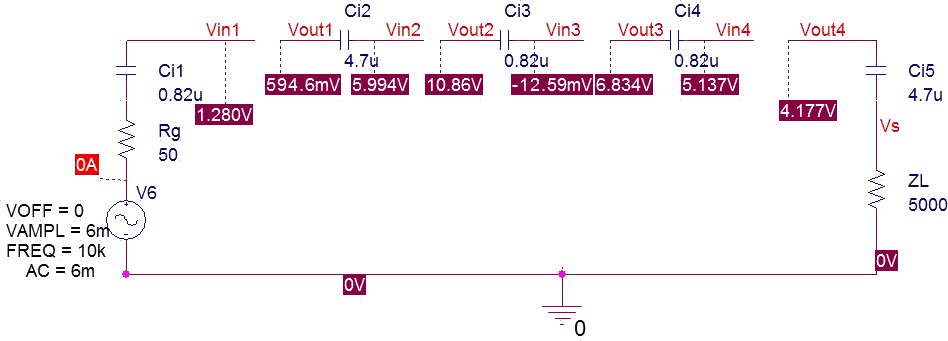
\includegraphics[width=17cm]{images/g}

    On choisit les autres condensateurs de manière à nous assurer une fréquence de coupure voisine de 100 \hertz.

   \subsection{Premier étage : Collecteur Commun}
    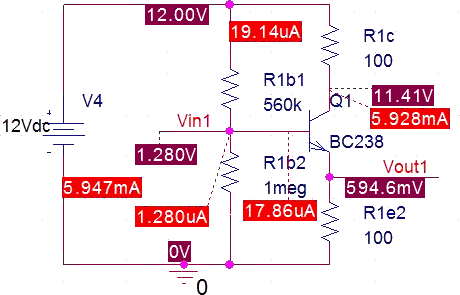
\includegraphics[width=17cm]{images/1}

   \subsection{Deuxième étage : Émetteur Commun}
    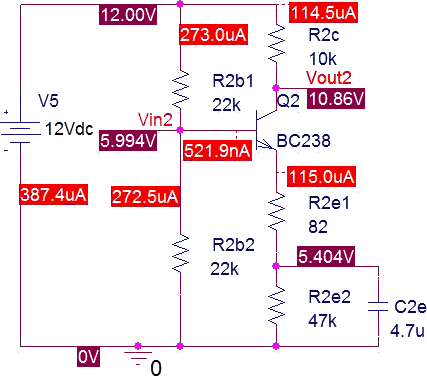
\includegraphics[width=17cm]{images/2}

   \subsection{Troisième étage : Amplificateur Différentiel}
    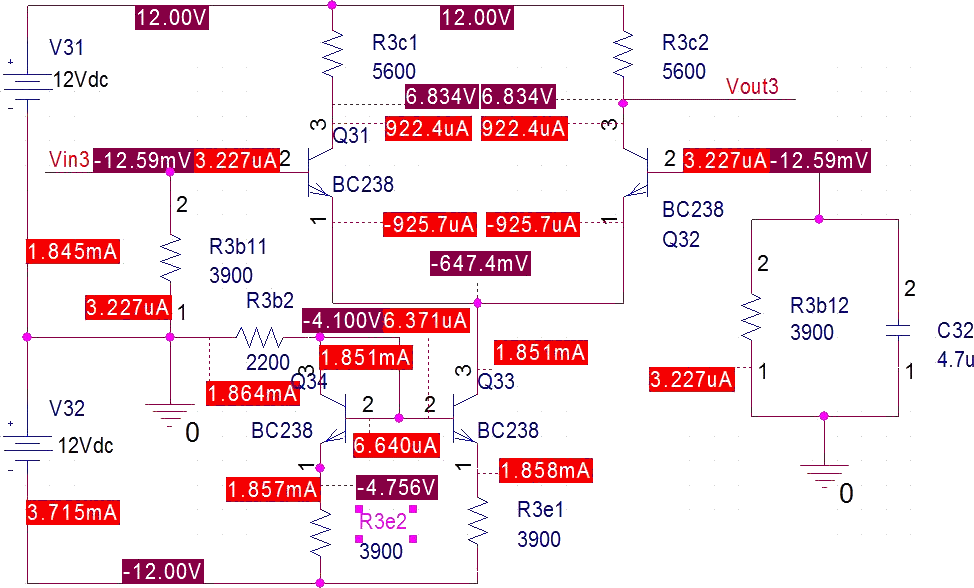
\includegraphics[width=17cm]{images/3}

   \subsection{Quatrième étage : Collecteur Commun}
    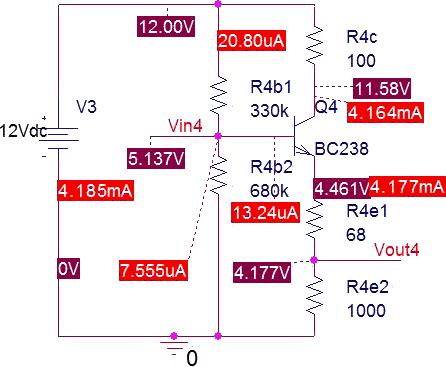
\includegraphics[width=17cm]{images/4}

  \section{Simulation}
   \subsection{Diagramme de Bode}
    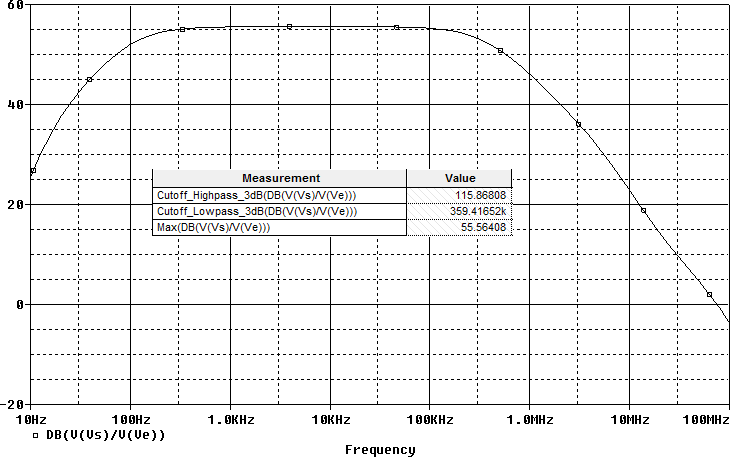
\includegraphics[width=17cm]{images/bode}

  \section{Respect du cahier des charges}
   Voici les caractéristiques principales de noter amplificateur, telles que données par
   Spice, qui complètent les données de polarisation présentes sur les schémas:

   \subsection{Fréquences de coupure}
    Ces fréquences sont données par Spice avec les fonctions \verb|Cutoff_Lowpass_3dB()| et \verb|Cutoff_Highpass_3dB()| :

    $F_{CBF} = 115$ \hertz

    $F_{CHF} = 359$ \kilo\hertz

   \subsection{Impédances d'entrée et de sortie}
    En traçant un "diagramme de Bode" sous Spice avec, pour chaque étage, $\cfrac{V_E}{I_E}$, on obtient (à 30 \kilo\hertz):
    \begin{itemize}
     \item $Z_{E_1} = \verb|32030|\ohm = Z_E$ : On respecte bien le cahier des charges.
     \item $Z_{E_2} = \verb|9644|\ohm$
     \item $Z_{E_3} = \verb|3294|\ohm$
     \item $Z_{E_4} = \verb|124060|\ohm$
    \end{itemize}

    Pour l'impédance de sortie, il faut modifier un peu le circuit sous spice : court-circuiter l'entrée et déplacer le générateur à la place de la charge. On obtient alors :
    \begin{itemize}
     \item $Z_{S_3} = \verb|5435|\ohm$
     \item $Z_{S_4} = \verb|85|\ohm = Z_S \Rightarrow$ Contrairement à ce que nous avions prévu, nous n'ajouterons pas de résistance série.
    \end{itemize}

   \subsection{Gain et dynamique de sortie}
    On obtient un gain de \verb|55,56| dB, soit une amplification de 600.
    Notre dynamique de sortie est de \verb|6,09012|\volt.
   \subsection{Distorsion harmonique}
    Toujours d'après Spice : \verb|TOTAL HARMONIC DISTORTION =   4,509345E+00 PERCENT|

   \subsection{Courants de collecteur}
    \begin{itemize}
     \item $I_{C_1} = 5,928 \milli\ampere$
     \item $I_{C_2} = 0,114 \milli\ampere$
     \item $I_{C_3} = 0,926 \milli\ampere$
     \item $I_{C_4} = 4,164 \milli\ampere$
    \end{itemize}

   \subsection{Amplitudes crête à crête}
    \begin{itemize}
     \item $A_1 =$ \verb|11,34| \milli\volt
     \item $A_2 =$ \verb|90,94| \milli\volt
     \item $A_3 =$ \verb|6,67| \volt
     \item $A_4 =$ \verb|6,09| \volt
    \end{itemize}

  \chapter{Bilan intermédiaire}
  \section{Respect du cahier des charges}
    \begin{tabular}{|l|l|c|c|c|c|c|}
     \hline
     & & Typique & Tolérance & Minimum & Maximum  & Obtenu\\
     \hline
     \multirow{4}{3cm}{Caractéristiques générales à 30k\hertz} & Gain en tension & 60 & $\pm$ 5dB & 55 & 65 & 55,56\\
     \cline{2-7} & Résistance d'entrée & 30 & $\pm$ 15 \% & 25,5 & 34,5 & \textcolor{green}{32}\\
     \cline{2-7} & Résistance de sortie & 100 & $\pm$ 15 \% & 85 & 115 & 85\\
     \cline{2-7} & Dyn. de sortie (5\kilo\ohm)& & & 6 & & 6,09\\
     \cline{2-7} & Dyn. de sortie (100\ohm)& & & 0,1 & & \textcolor{green}{2,02}\\
     \hline
     \multirow{2}{3cm}{Fréquence de coupure} & basse & 100 & $\pm$ 20 \% & 80 & 120 & \textcolor{green}{115}\\
     \cline{2-7} & haute & & & 500 & & \textcolor{red}{363}\\
     \hline
     Distorsion harmonique & [1k\hertz;100k\hertz] & & & & 5,00 \% & 4,5\\
     \hline
     \multirow{2}*{Tension d'alimentation} & Positive & 12V & & 0 & 12 & 12\\
     \cline{2-7} & Négative & -12V & & -12 & 0 & -12\\
     \hline
     Courant de collecteur & & & & 0,1 & 10 & \textcolor{green}{0,11 à 5,9}\\
     \hline
    \end{tabular}

\end{document}
